\chapter{Estado del arte\label{cap:estadoDelArte}}

En este capítulo se presenta la única plataforma de captura y reproducción de tráfico de red que se basa en la misma \gls{FPGA} que este Trabajo de Fin de Grado, \textit{The Open Source Network Tester}.
Adicionalmente, se exponen también (brevemente) otras herramientas similares de captura, reproducción y análisis.
Se intenta por tanto detallar de forma objetiva los aspectos positivos y las carencias de las distintas alternativas, poniendo así en contexto el proyecto a desarrollar.
Dado que la naturaleza de este proyecto es desarrollar una interfaz web, se hace especial hincapié en la interfaz de usuario de la que dispone cada uno de los sistemas analizados.

\section{The Open Source Network Tester\label{sec:eda:osnt}}

\textit{The Open Source Network Tester (OSNT)}~\cite{osnt} es un generador y capturador de tráfico.
Se ejecuta sobre cuatro \textit{NetFPGA-10G} (el mismo modelo de sonda que el seleccionado en este proyecto).
Permite generar o capturar paquetes de todo tipo de tamaño, y establecer la tasa a la que se realizan estas operaciones.

Pros
- Open source
- Interfaz gráfica
- Muchas opciones y configurable
OSNT IS LOW-COST
OSNT IS BASED ON THE NETFPGA-10G PLATFORM AND A 4X10GB/S SYSTEM CAN BE BUILT FOR LESS THAN 2,000k.
OSNT IS OPEN-SOURCE
ALL THE HARDWARE AND SOFTWARE DESIGNS ARE FREELY AVAILABLE FOR YOU TO USE AND EXTEND.
OSNT WORKS OUT OF THE BOX
OSNT COMES WITH SOME STANDARD LIBRARIES FOR GENERATING AND CAPTURING USER-SELECTED PACKET LENGTHS AT DIFFERENT RATES.
OSNT IS EXTENSIBLE
IT IS EASY TO ADD YOUR OWN PACKET FORMATS, OR EXTEND OSNT TO ADD NEW PROTOCOLS.
OSNT IS A STARTING POINT
WE DEVELOPED OSNT AS A COMMUNITY-OWNED PLATFORM TO ENABLE LOW-COST, SOPHISTICATED TESTING.
MULTIPLE OSNT SYSTEMS CAN BE SYNCHRONIZED
USE GPS TO SYNCHRONIZE HIGH-PRECISION TIMESTAMPS ACROSS MULTIPLE OSNT SYSTEMS.

Cons
- No da la tasa
- No monitoriza el sistema (trazas, tasa)
- Arquitectura
- Interfaz mala (no intuitiva, linux) > no es posible manejar desde fuera

\begin{figure}[!htp]
  \centering
  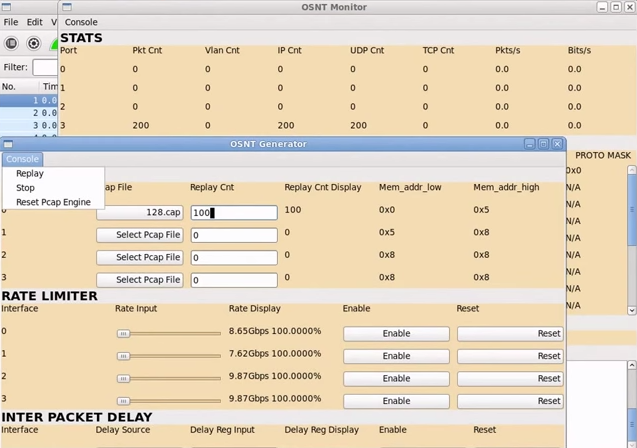
\includegraphics[width=0.7\textwidth,clip=true]{graphics/capturas/osnt}
  \caption{Captura de la interfaz gráfica de \textit{OSNT}.}
  \label{fig:osnt}
\end{figure}

\section{Otras herramientas similares\label{sec:eda:otras}}

\subsection*{tcpdump y libpcap\label{sec:eda:tcpdump}}

La utilidades \textit{tcpdump} y \textit{libpcap}~\cite{tcpdump}, implementadas como librerías, permiten analizar el tráfico que circula por la red.
Así, el usuario puede capturar y mostrar en tiempo real los paquetes transmitidos y recibidos en una red a la que el ordenador esté conectado.
Se suele utilizar para depurar aplicaciones que envían y reciben tráfico de red, aunque tiene otros usos como leer datos no cifrados enviados por otros ordenadores.

Estas librerías poseen otras características adicionales que las hacen interesantes.
Por un lado, son de código libre y tienen una comunidad detrás que añade funcionalidad y corrige errores de forma continua.
Por otra parte, da la posibilidad de aplicar filtros sobre las capturas, seleccionando los paquetes que se considere oportuno.
Desde el punto de vista de interfaz de usuario, \textit{tcpdump} y \textit{libpcap} se manejan desde la línea de comandos.
Esto hace más complicado empezar a capturar tráfico de red si no se tienen conocimientos previos de las herramientas.

\subsection*{Wireshark\label{sec:eda:wireshark}}

\textit{Wireshark}~\cite{wireshark} es un analizador de protocolos de red.
Provee una funcionalidad similar a la de \textit{tcpdump}, añadiendo una interfaz gráfica y más opciones de filtrado de la información.
Así, permite o bien ver todo el tráfico en tiempo real que pasa a través de una red (almacenándolo opcionalmente), o bien analizar tráfico ya capturado anteriormente.

Una de las ventajas de \textit{Wireshark} es que soporta casi todos los protocolos de red, y permite de manera sencilla añadir protocolos adicionales.
Otra es que, al contrario que \textit{tcpdump} y \textit{libpcap}, cuenta con una interfaz gráfica de usuario para manejar la captura y reproducción.
Sin embargo, esta interfaz no es demasiado intuitiva, y para el uso de filtros se requiere la consulta del manual.

\subsection*{Detect-Pro\label{sec:eda:detectpro}}

\textit{Detect-Pro}~\cite{detectpro} es una herramienta modular de análisis pasivo (sin intervenir).
Analiza todo el tráfico de un enlace de red paquete a paquete, proporcionando series temporales de tráfico, análisis a nivel de flujo, análisis de tendencias y recolección selectiva de \glspl{traza}.
Identifica así patrones de actividad, detectando anomalías mediante estos mismos patrones.

Esta herramienta cuenta con una interfaz web intuitiva, por lo que puede ser manejada sin demasiadas complicaciones.
No obstante, no está enfocado tanto a la captura y reproducción de tráfico de red sino a su análisis, por lo que se desvía un poco del propósito planteado.
Por último, es un producto que requiere ser contratado, siendo por tanto su público no tan amplio como el resto de herramientas analizadas.

\section{Conclusiones\label{sec:eda:conclusiones}}

TODO: Conclusiones
  - Pensadas para analizar, mucha más funcionalidad de la que se necesita en este problema

Carencias principales:
  - Demasiada funcionalidad no aprovechada por el usuario
  - Usabilidad (interfaz)
  - Disponibilidad (mismo servidor, no remoto)
Arquitectura no está pensada para el manejo por usuarios
